\documentclass[a4paper,10pt,english]{article}
\usepackage[utf8]{inputenc}
\usepackage[norsk]{babel}
\usepackage{amsmath,graphicx,varioref,verbatim,amsfonts,geometry}
\usepackage[usenames,dvipsnames,svgnames,table]{xcolor}
\usepackage[colorlinks]{hyperref}
\usepackage{pdfpages}
\setlength{\parindent}{0mm}
\setlength{\parskip}{1.5mm}
\usepackage{textcomp}
\usepackage{xcolor}
\usepackage{textcomp}
\usepackage{listings}
\definecolor{listinggray}{gray}{0.9}
\definecolor{lbcolor}{rgb}{0.9,0.9,0.9}
\usepackage{xparse}
\renewcommand{\thesubsection}{\alph{subsection}}
\usepackage{titling}
\setlength{\droptitle}{-4em}
\addtolength{\hoffset}{-0.5in}
\addtolength{\textwidth}{0.75in}
\addtolength{\voffset}{-.5in}
\addtolength{\textheight}{1.75in}

\NewDocumentCommand{\codeword}{v}{%
\texttt{\textcolor{blue}{#1}}%
}

\lstset{
 backgroundcolor=\color{lbcolor},
 tabsize=4,
 rulecolor=,
 language=matlab,
 basicstyle=\scriptsize,
 upquote=true,
 aboveskip={1.5\baselineskip},
 columns=fixed,
 showstringspaces=false,
 extendedchars=true,
 breaklines=true,
 prebreak = \raisebox{0ex}[0ex][0ex]{\ensuremath{\hookleftarrow}},
 frame=single,
 showtabs=false,
 showspaces=false,
 showstringspaces=false,
 identifierstyle=\ttfamily,
 keywordstyle=\color[rgb]{0,0,1},
 commentstyle=\color[rgb]{0.133,0.545,0.133},
 stringstyle=\color[rgb]{0.627,0.126,0.941},
}
\title{Project 1
}
\author{Bernt Jonas Fløde
}
\begin{document}
\maketitle

\section*{Bevis for omskriving (1a)}

Vil vise at
\begin{equation*} \mathbf{A} \mathbf{v} = h^2 \mathbf{f},\end{equation*}eller
\begin{equation*} \mathbf{A} \mathbf{v} / h^2 = \mathbf{f}\end{equation*}
Ved å skrive ut $-\mathbf{A} \mathbf{v} / h^2$, får vi
\begin{equation*}-\frac{v_2-2v_1}{h^2} = f_1\hspace{0.5cm}\mathrm{for}\hspace{0.1cm}i=1,\dots, n,\end{equation*}\begin{equation*}-\frac{v_3+v_1-2v_2}{h^2} = f_2\hspace{0.5cm}\mathrm{for}\hspace{0.1cm}i=1,\dots, n,\end{equation*}\begin{equation*}-\frac{v_4+v_2-2v_3}{h^2} = f_3\hspace{0.5cm}\mathrm{for}\hspace{0.1cm}i=1,\dots, n,\end{equation*}og så videre, med det siste leddet
\begin{equation*}-\frac{v_{n-1}-2v_n}{h^2} = f_n\hspace{0.5cm}\mathrm{for}\hspace{0.1cm}i=1,\dots, n,\end{equation*}
Mer kompakt betyr dette det samme som
\begin{equation*}-\frac{v_{i+1}+v_{i-1}-2v_i}{h^2} = f_i\hspace{0.5cm}\mathrm{for}\hspace{0.1cm}i=1,\dots, n,\end{equation*}som er definisjonen av den andrederivertes tilnærming.

Altså vil den kontinuerlige ekvivalenten til dette uttrykket være
\begin{equation*}-u''(x) = f(x),\end{equation*}som var utgangspunktet for utledningen, og beviset er ferdig.

\section*{Algoritme for tridiagonale}

Vi skal her løse ligningen $\mathbf{A} \mathbf{v} = \mathbf{\tilde{b}}$ med hensyn på $\mathbf{v}$. Det gjør vi ved å radredusere matrisen $[\mathbf{A}\hspace{0.1cm}\mathbf{\tilde{b}}]$, vi skal da få $[\mathbf{I}\hspace{0.1cm}\mathbf{v}]$ der $\mathbf{I}$ er identitetsmatrisen.

Altså skal vi radredusere følgende matrise:

\[
    \begin{bmatrix}
        b_1& c_1 & 0 &\dots   & \dots &\dots &\tilde{b}_1 \\
        a_1 & b_2 & c_2 &\dots &\dots &\dots &\tilde{b}_2 \\
        0 & a_2 & b_3 & c_3 & \dots & \dots &\dots \\
        & \dots   & \dots &\dots   &\dots & \dots &\dots \\
        &   &  &a_{n-2}  &b_{n-1}& c_{n-1} &\dots \\
        &    &  &   &a_{n-1} & b_n &\tilde{b}_n \\
    \end{bmatrix}
\]

For å gjøre notasjonen lettere senere setter vi $b_1 = \beta_1$ og $\tilde{b}_1 = \tilde{\beta}_1$, slik at matrisen er:

\[
    \begin{bmatrix}
        \beta_1& c_1 & 0 &\dots   & \dots &\dots &\tilde{\beta}_1 \\
        a_1 & b_2 & c_2 &\dots &\dots &\dots &\tilde{b}_2 \\
        0 & a_2 & b_3 & c_3 & \dots & \dots &\dots \\
        & \dots   & \dots &\dots   &\dots & \dots &\dots \\
        &   &  &a_{n-2}  &b_{n-1}& c_{n-1} &\dots \\
        &    &  &   &a_{n-1} & b_n &\tilde{b}_n \\
    \end{bmatrix}
\]

Vi starter radreduksjonen med å få vekk $a$-ene. For å radredusere vekk $a_1$, kan vi gjøre II: II - $a_1$/I (dvs. vi regner ut $a_1$ delt på hvert tall i første raden, og trekker resultatet fra tilsvarende tall i andre rad). Da får vi følgende matrise:

\[
    \begin{bmatrix}
        \beta_1& c_1 & 0 &\dots   & \dots &\dots &\tilde{\beta}_1 \\
        0 & \beta_2 & c_2 &\dots &\dots &\dots &\tilde{\beta}_2 \\
        0 & a_2 & b_3 & c_3 & \dots & \dots &\dots \\
        & \dots   & \dots &\dots   &\dots & \dots &\dots \\
        &   &  &a_{n-2}  &b_{n-1}& c_{n-1} &\dots \\
        &    &  &   &a_{n-1} & b_n &\tilde{b}_n \\
    \end{bmatrix}
\]

der $\beta_2 = b_2 - a_1/c_1$ og $\tilde{\beta_2} = \tilde{b}_2 - a_1/\tilde{\beta_1}$.

Ved å fortsette slik for $\beta_{i+1} = b_{i+1} - a_i/c_i$ og $\tilde{\beta}_{i+1} = \tilde{b}_{i+1} - a_i/\tilde{\beta}_i$, får vi følgende matrise:

\[
    \begin{bmatrix}
        \beta_1& c_1 & 0 &\dots   & \dots &\dots &\tilde{\beta}_1 \\
        0  & \beta_2 & c_2 &\dots &\dots &\dots &\tilde{\beta}_2 \\
           &\dots& \beta_3 & c_3 & \dots & \dots &\dots \\
        &   & \dots &\dots   &\dots & \dots &\dots \\
        &   &  &  &\beta_{n-1}& c_{n-1} &\dots \\
        &    &  &   & & \beta_n &\tilde{\beta}_n \\
    \end{bmatrix}
\]

Fra teorien i lineær algebra kan vi nå se hva svaret må bli. Den nederste raden forteller at $\beta_n v_n = \tilde{\beta}_n$, altså $v_n = \tilde{\beta}_n/\beta_n$. Raden over forteller at $\beta_{n-1} v_{n-1} + c_{n-1} v_n = \tilde{\beta}_{n-1}$, altså $v_{n-1} = \frac{\tilde{\beta}_{n-1} - c_{n-1} v_n}{\beta_{n-1}}$. Generelt forteller en rad at $\beta_i v_i + c_i v_{i+1} = \tilde{\beta}_i$, altså $v_i = \frac{\tilde{\beta}_i - c_i v_{i+1}}{\beta_i}$, og hvis vi setter $v_{n+1} = 0$ er sistnevnte formel også gyldig for $i = n$.

Oppsummert kan vi finne svaret med de tre rekursive formlene
$$\beta_{i+1} = b_{i+1} - a_i/c_i$$
$$\tilde{\beta}_{i+1} = \tilde{b}_{i+1} - a_i/\tilde{\beta}_i$$
$$v_i = \frac{\tilde{\beta}_i - c_i v_{i+1}}{\beta_i}$$
med initialbetingelsene $b_1 = \beta_1$, $\tilde{b}_1 = \tilde{\beta}_1$ og $v_{n+1} = 0$.

I C++ kan dette implementeres ved hjelp av for-løkker. De to første rekursive formlene implementeres i en forlengs for-løkke, mens den siste implementeres i en baklengs for-løkke. De to første initialbetingelsene gis direkte i koden, mens den siste er implisitt gitt i C++. Koden blir slik:

\begin{lstlisting}
beta[1]       = b[1];
beta_tilde[1] = b_tilde[1];
for (int i=1; i<n; i++) {
	a_div_beta = a[i] / beta[i];
	beta[i+1]       = b[i+1]    - a_div_beta * c[i];
	beta_tilde[i+1] = beta[i+1] - a_div_beta * beta_tilde[i];
}
for (int i=n; i>0; i--) {
	v[i] = (beta_tilde[i] - c[i] * v[i+1]) / (b_tilde[i]);
}
return v;
\end{lstlisting}

der \codeword{a_div_beta} er en hjelpevariabel som sparer programmet fra å regne ut dette to ganger, og dermed gjøre programmet raksere.

\begin{figure}[h!]
	\centering
	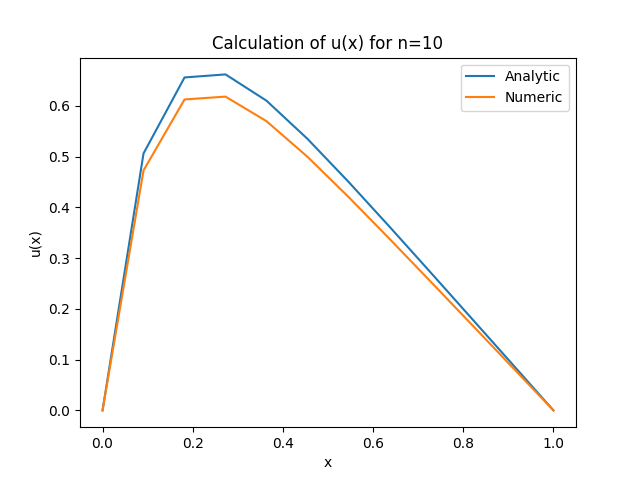
\includegraphics[width=10cm]{plots/tridiagonal_n=10.png}
	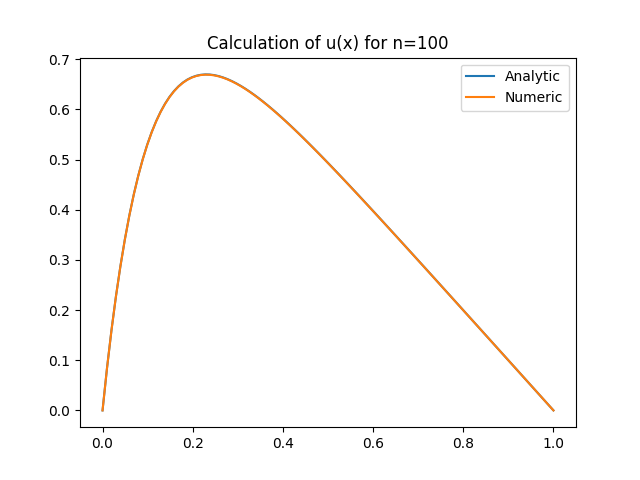
\includegraphics[width=10cm]{plots/tridiagonal_n=100.png}
	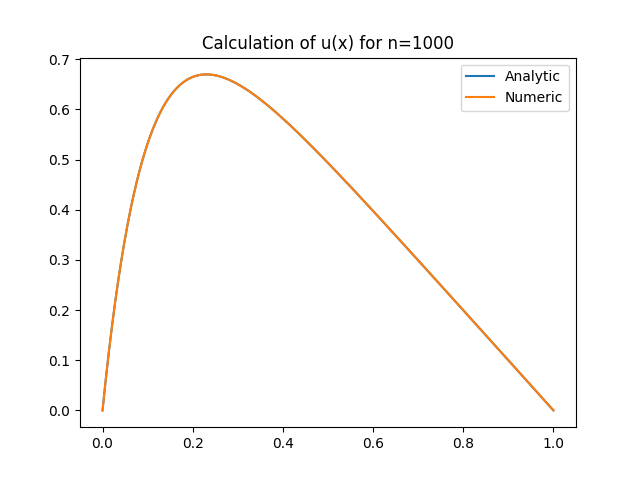
\includegraphics[width=10cm]{plots/tridiagonal_n=1000.png}
	\caption{Analytisk og numerisk løsning av differensialligning for n=10, n=100 og n=1000.}
	\label{fig:tridiagonal}
\end{figure}

Hvis vi ser på koden er det åtte flyttallsoperasjoner inne i for-løkkene, som vi si at tiden som utregningen bruker går som $8\hspace{0.1cm}n$.

Denne koden finnes også i dataprogrammet \codeword{tridiagonal.cpp} lenger ned. Dataprogrammet finner en numerisk løsning av $-u''(x)=f(x)$ der $f(x)=100 e^{-10x}$ som er funnet med metoden som her har blitt beskrevet, og sammenligner det med den analytiske løsningen $u(x)=1-(1-e^{-10}) x-e^{-10x}$. Dette gjør det for $n=10$, $n=100$ og $n=1000$, se figur \ref{fig:tridiagonal}.

\subsection*{Spesialtilfelle}
Vi ser nå på et spesialtilfelle der $a_i=a$, $b_i=b$ og $c_i=c$ for alle $i$, for tre gitte tall $a$, $b$ og $c$. Da er det mulig å forenkle dataprogrammet ved å gjøre om arrayene \codeword{a}, \codeword{b} og \codeword{c} til enkle flyttall. Det er også nærliggende å tro at det skulle være mulig med flere forenklinger i koden får å få den til å gå enda raskere, men noen slik forenkling har jeg ikke funnet. Tiden som utregningen bruker går altså fortsatt som $8\hspace{0.1cm}n$. Koden blir slik:

\begin{lstlisting}
beta[1]       = b;
beta_tilde[1] = b_tilde[1];
for (int i=1; i<n; i++) {
	a_div_beta = a / beta[i];
	beta[i+1]       = b         - a_div_beta * c;
	beta_tilde[i+1] = beta[i+1] - a_div_beta * beta_tilde[i];
}
for (int i=n; i>0; i--) {
	v[i] = (beta_tilde[i] - c * v[i+1]) / (b_tilde[i]);
}
return v;
\end{lstlisting}

Her er tabellen som blir skrevet ut:

\input{out/project1d_table.dat}

Vi ser at nøyaktigheten blir bedre og bedre for mindre $h$, fram til et punkt der avrundingsfeil blir dominerende.

tridiagonal.cpp
\lstinputlisting{tridiagonal.cpp}
\section*{LU-dekomposisjon}
Prøver også å skrive et program for ordinært LU-dekomposisjon til å løse de samme ligningene som over. Dette er ventet å bruke mer tid fordi det er flere flyttallsoperasjoner. Dessuten får programmet en feilmelding som je*/g ikke vet hvordan kan løses.

LU.cpp
\lstinputlisting{LU.cpp}
\section*{Annet kode}
Følgende Python-program blir brukt til å kjøre de andre programmene:
project1.py
\lstinputlisting{project1.py}

\end{document}
\grid
